\section{Problemformulering}
Tracking af en lerdue i English Skeet \todo[inline, author=Anders]{eventuelt starte med en liste over forkortelser}(ES) vha. PTS. 
Lerduen er i vores opstilling udskiftet med en bold, men ellers følges reglerne for ES.
\todo[color=yellow! 100, inline, author=Anders]{Henvisning til litteraturliste eller fodnote}
Bolden bevæger sig i et 3D rum med negligerbar luftmodstand. \\

\begin{figure}[th!]
\centering
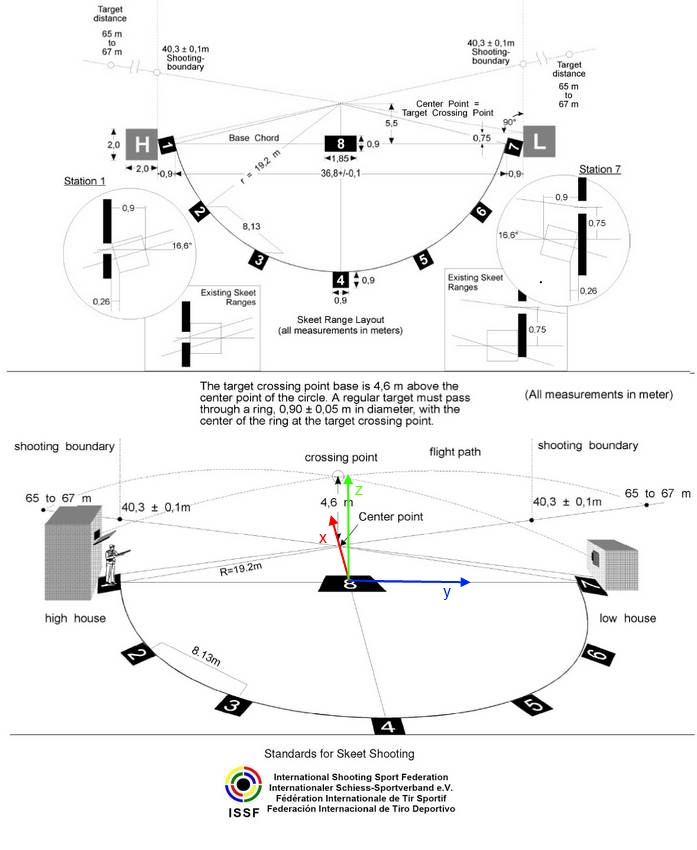
\includegraphics[width=0.4\textwidth]{./graphics/skeet-diagram_med_akser}
\caption[tekst i indholdsfortegnelsen]{figurtekst}
\label{fig:ES}
\end{figure}	
Systemets input er 60 kartesisiske koordinatsæt (x,y,z) per sekund. Hvor disse 
koordinater stammer fra, er uden for projektafgrænsningen. \\

Systemet dimensioneres til brug ifbm. en konkurrence i ES. En skitse over 
banen ses på figur \ref{fig:ES}. Det kartesiske koordinatsystem har origo i halvcirklens centrum, 
som indtegnet \todo[inline, author=Michael]{De er så indtegnet forkert.. Flot arbejde, klaphat..} 
nederst på figuren. I ES skal rammes serier af duer/mål der afskydes fra 
enten ”High House” eller ”Low House”, og med skud fra hver af de otte stationer langs 
cirkelperiferien. I dette projekt kigges kun på tilfældet hvor der afskydes mål fra ”High-
House” med pan-and-tilt systemet placeret på station 4.\\

Jævnfør reglerne for ES, skal duer/mål passere target crossing point (TCS) som er 
placeret i $4,57 [m]$ over origo. (0; 0; 4.57). Fejlmargin for passagen er $\pm0,45 [m]$. 
Målene skal desuden flyve $50 – 52 [m]$.  High house er placeret $20,11 [m]$ fra TCS, i en 
højde af $3,05 [m]$. Da luftmodstanden er negligerbar kan parablen (2. grads 
polynomium) findes ved at indsætte de kendte punkter. Herunder er parablen vist i et 
2D plan, figur \ref{fig:HH2D_para}.
\begin{figure}[!th]
\centering
\begin{tikzpicture}[scale=1]
\include*{./graphics/high_house_2D_parabola}
\end{tikzpicture}
\caption[Lerdue parabel]{Viser parablen af lerduens bane.}
\label{fig:HH2D_para}
\end{figure}
\todo[inline, author=Anders]{Den rigtige funktion skal sættes ind, afventer Michael}




Målet bliver affyret med en hastighed på $34 [m/s]$, i en vinkel på $9^{\circ}$ ift. xy-
planet. Set ovenfra bevæger målet sig som set på figur \ref{fig:para_in_xy_plane}. 
Figuren ses nedslagspunktet fra High-House, der er i alt $52 [m]$ startpositionen samt 
PTS placering i punktet B. 



\begin{figure}[!th]
\centering
\begin{tikzpicture}[scale=1]
\include*{./graphics/parabola_in_xy_plane}
\end{tikzpicture}
\caption[tekst i indholdsfortegnelsen]{figurtekst}
\label{fig:para_in_xy_plane}
\end{figure}

\todo[inline, author=Anders]{Jeg er gået igang med at tegne den og den kommer in snart.}